\section{Case study: EKF tracking}
\label{sec:EKF}
The proposed approximate computing algorithm is evaluated for a non-linear, Gaussian, single-target tracking problem. It is assumed that the target is circularly rotating over the $xy$-plane. To have the paper self-contained and to simplify explaining the points at which approximation is imposed, the motion model and EKF equations are detailed in this section.

It is assumed that the sensor measures the range and bearing (azimuth) of the target in meters and radians, respectively. This is a typical sensing scenario in LiDAR, radar and stereo vision used in numerous applications, e.g., autonomous vehicles \cite{7398055},

\begin{equation}
\left\{
\begin{array}{l}
r_k = \sqrt{\bar{x}_k^2 + \bar{y}_k^2} + n_{r_k} \\
\phi_k = atan2(\bar{y}_k, \bar{x}_k) + n_{\phi_k}
\end{array}
\right.,
\label{eq:Meas}
\end{equation}

\noindent where $\bar{x}_k$ and $\bar{y}_k$ are the true states of the target location, ${\bf Z}_k = [r_k, \phi_k]$ contains the measured range and bearing values, and ${\bf N}_k = [n_{r_k}, n_{\phi_k}]$ is a random vector sampled from a Gaussian with zero mean, and all are at the $k^{th}$ iteration. $atan2(.)$ computes the angle between the point (vector) $[\bar{x}_k, \bar{y}_k]$ and positive $x$-axis.

\begin{figure}[tb]
  \centering
  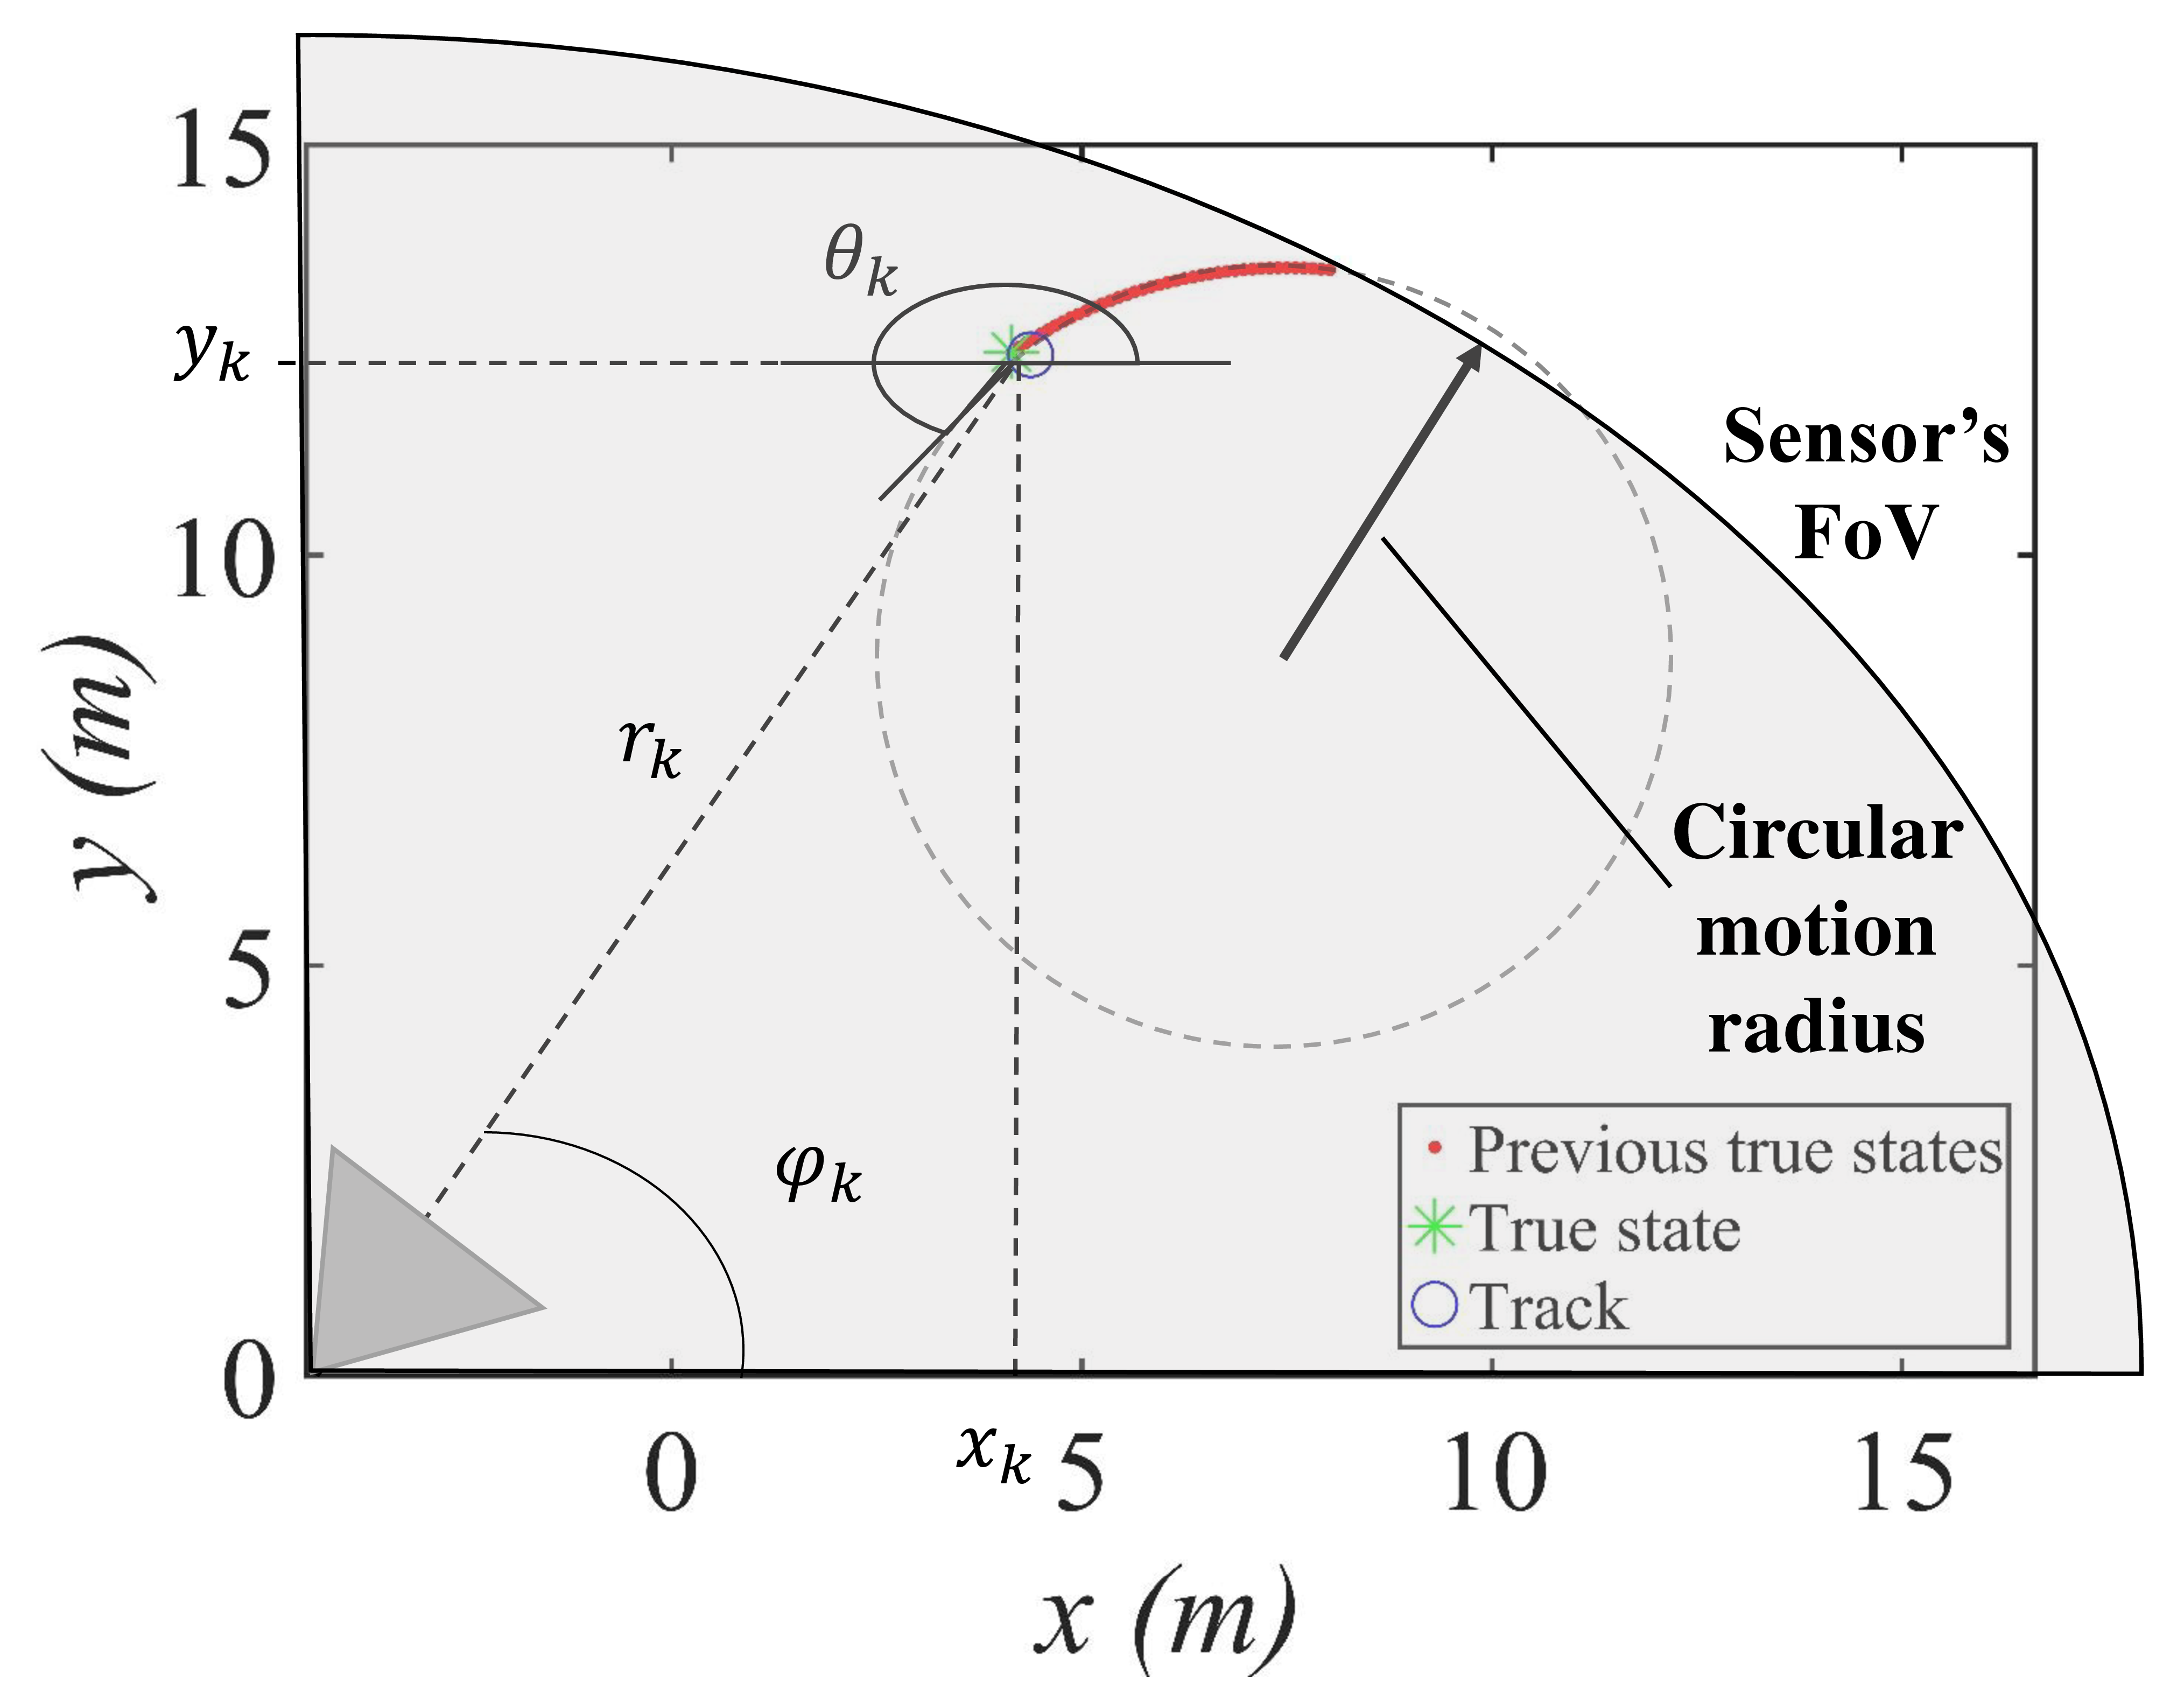
\includegraphics[width=0.95\columnwidth]{img/Trackingfinal.png}
  \caption{The tracking scene containing the FoV of the sensor, target motion trajectory and state parameters definition.}
  \label{fig:TrackScene}
\end{figure}

It is assumed that at time $k$, the target has a three dimensional state vector ${\bf X}_k = [x_k, y_k, \theta_k]^\intercal$, in which $[x_k, y_k]$ and $\theta_k$ are the position and pose states of the target, respectively. This is shown in Fig.~\ref{fig:TrackScene}. The state estimation equations are,

\begin{equation}
\left\{
\begin{array}{l}
\hat{x}_k = x_{k-1} + (\Delta t) v_k \cos(w_k \Delta t + \theta_{k-1}) + m_{x_k} \\
\hat{y}_k = y_{k-1} + (\Delta t) v_k \sin(w_k \Delta t + \theta_{k-1}) + m_{y_k} \\
\hat{\theta}_k = \theta_{k-1} + w_k \Delta t + m_{\theta_k}
\end{array}
\right..
\label{eq:State}
\end{equation}

\noindent ${\bf u}_k = [v_k, w_k]$ is the speed vector containing the radial and angular speed parameters in m$/$sec and rad$/$sec, respectively, which can be computed from previous state vectors. $\Delta t$ is the time update resolution in seconds. $\hat{{\bf X}}_k = [\hat{x}_k, \hat{y}_k, \hat{\theta}_k]^\intercal$ is the estimated state vector for the $k^{th}$ iteration. ${\bf M}_k = [m_{x_k}, m_{y_k}, m_{\theta_k}]^\intercal$ is a random vector sampled from a Gaussian distribution with zero mean. 

Due to the non-linearity in (\ref{eq:Meas}) and (\ref{eq:State}), Gaussianity will not be preserved and therefore, a linear approximation is used based on Taylor series expansion. 
The Jacobian matrix for the estimation step is computed using \ref{eq:State} as follows:

\begin{equation}
{\bf J}_{X, k-1} = \left[
\begin{array}{llr}
1 & 0 & -(\Delta t) v_k \sin(w_k \Delta t + \theta_{k-1}) \\
0 & 1 &  (\Delta t) v_k \cos(w_k \Delta t + \theta_{k-1}) \\
0 & 0 & 1 
\end{array}
 \right].
\end{equation}

\noindent Assuming ${\bf \Sigma}_{{X}, k-1}$ and ${\bf Q}_{k}$ are the state and noise covariance matrices at $k-1$ and $k$, the estimated state covariance matrix at iteration $k$ will be: ${\bf \Sigma}_{\hat{X}, k} = {\bf J}_{X, k-1}{\bf \Sigma}_{X, k-1}{\bf J}_{X, k-1}^\intercal + {\bf Q}_{k}$.

The correction step of EKF incorporates the measurement at time $k$. Let ${\bf R}_k$ be the measurement covariance matrix. Then the corrected state vector can be computed as follows,

\begin{equation}
\begin{array}{l}
{\bf X}_{k} = \hat{{\bf X}}_k + {\bf K}_k ({\bf Z}_k - h(\hat{{\bf X}}_k)) \\
{\bf K}_k = {\bf \Sigma}_{\hat{X}, k} {\bf H}_k^\intercal {\bf S}_k^{-1} \\
{\bf S}_k = {\bf H}_k {\bf \Sigma}_{\hat{X}, k} {\bf H}_k^\intercal + {\bf R}_k
\end{array}.
\end{equation}

\noindent ${\bf K}_k$ is the Kalman gain, ${\bf S}_k$ is the innovation covariance and ${\bf X}_{k}$ is the (corrected) state vector at the $k^{th}$ iteration. $h(.)$ is a non-linear function, which maps the current estimated target state to the coordinate frame of the sensor. ${\bf H}_k$ is the measurement's Jacobian matrix, which is computed as follows using \ref{eq:Meas},

\begin{equation} 
{\bf H}_k = 
\frac{1}{\sqrt{x_k^2 + y_k^2}}
\left[
\begin{array}{lll}
x_k & y_k & 0 \\
-y_k & x_k & 0
\end{array}
\right].
\end{equation}

\noindent The corrected covariance matrix for the $k^{th}$ iteration will then be,

\begin{equation}
{\bf \Sigma}_{X, k} = 
\left(
\left[
\begin{array}{lll}
1 & 0 & 0 \\ 
0 & 1 & 0 \\
0 & 0 & 1 
\end{array}
\right]
- {\bf K}_k {\bf H}_k
\right)
{\bf \Sigma}_{\hat{X}, k}.
\label{eq:correctCOV}
\end{equation}

\subsection{KL divergence for Gaussian motion}
Comparison with the prior knowledge can be performed in various ways. 
For an iterative filtering, which estimates and corrects the state of the object using the obtained measurements, the prior knowledge can be defined using the target's motion. Any deviation from this known model can be used to compromise over approximation during run-time. 

One solution to quantify such model is to stack state vectors for a given number of consecutive iterations. Then estimating the statistics of the stacked tracks, using either parametric or non-parametric approaches, can be used to map the result to our prior knowledge. 

To be more specific, in this paper, we use a parametric approach to approximate the probability density function (PDF) of the stacked target states from iteration $k$ to $k+N$, i.e. ${\bf s}_{k:k+N}$. 
Our prior knowledge is then compared with the computed approximated PDF. In our work, we use KL divergence to perform this task as follows,

\begin{equation}
D_{KL}({\bf H}_{k, N} || {\bf H}_{p}) = \sum_{i}{{\bf H}_{k, N}} \log{\frac{{\bf H}_{k, N}}{{\bf H}_{p}}}
\label{eq:KLDIV1}
\end{equation}

\noindent in which ${\bf H}_{k, N}$ is the approximated PDF of the $k^{th}$ to $(k+N)^{th}$ state samples and ${\bf H}_{p}$ is the "prior knowledge" PDF of the target's motion.

For this experimental setting, we assume that the object's motion statistics remains Gaussian (our prior knowledge). This can be iteratively evaluated by (\ref{eq:KLDIV1}). It can be easily shown that the KL divergence for two Gaussian distributions can be simplified as follows,

\begin{equation}
D_{KL}({\bf H}_{k, N} || {\bf H}_{p}) = \log{\frac{\sigma_p}{\sigma_{k, N}}} + \frac{\sigma_{k, N}^2 + (\mu_{k, N} - \mu_p)^2}{2\sigma_p^2} - \frac{1}{2}
\label{eq:KLDIV2}
\end{equation}

\noindent in which, ($\mu_{k, N}$, $\sigma_{k, N}^2$) and ($\mu_p$, $\sigma_p^2$) are the mean vector and variance of the stacked samples and prior knowledge, respectively. For our experiments, we assume that $\mu_p$ is the radius of the target's circular rotation, which is known with a $\pm \sigma_p$ standard deviation (both in meters).

We define the stacked samples ${\bf s}_{k:k+N}$ as the Euclidean distance between the target state $[x_k, y_k]^\intercal$ and centre of rotation.
The mean and variance $\mu_{k, N}$ and $\sigma_{k, N}^2$ are then computed as follows,

\begin{equation}
\begin{array}{l}
\mu_{k, N} = \frac{\sum_{i}{{s}^i_{k:k+N}}}{N} \\
\sigma_{k, N}^2 = \frac{\sum_{i}{({s}^i_{k:k+N}} - \mu_{k, N})^2}{N}
\end{array}
\end{equation}

\noindent in which, ${s}^i_{k:k+N}$ is the $i^{th}$ element in ${\bf s}_{k:k+N}$. Small values for $D_{KL}(.)$ correspond to higher similarity between the prior knowledge and tracks. Therefore, more intense approximation is imposed. On the other hand, the approximation level is reduced once the $D_{KL}(.)$ is higher than a given threshold.
